% This file demonstrates how to use the IEEEConf LaTeX2e macro package,
% to prepare a manuscript for proceedings on CD of the conference
% FedCSIS
%
\documentclass[conference]{IEEEtran}
%\documentclass[a4paper]{IEEEconf}

% This package serves to balance the column lengths on the last page of the document.
% please, insert \balance command in the left column of the last page

\usepackage{balance}

%% to enable \thank command
\IEEEoverridecommandlockouts 
%% The usage of the following packages is recommended
%% to insert graphics
%\usepackage[dvips]{graphicx}
% to typeset algorithms
\usepackage{algorithmic}
\usepackage{algorithm}
% to typeset code fragments
\usepackage{listings}
% to make an accent \k be available
\usepackage[OT4,T1]{fontenc}
% provides various features to facilitate writing math formulas and to improve the typographical quality of their output.
\usepackage[cmex10]{amsmath}
\interdisplaylinepenalty=2500
% por urls typesetting and breaking
\usepackage{url}
% for vertical merging table cells
\usepackage{multirow}

% \usepackage{graphicx}
\usepackage{epstopdf}
\usepackage{graphicx}


%\usepackage[T1]{fontenc}
%\usepackage[utf8]{inputenc}
%\usepackage[slovak]{babel}

\usepackage[slovak, english]{babel}

\usepackage{listings}             % Include the listings-package


% define environments for remarks and examples
\newtheorem{remark}{Remark}[section]
\newtheorem{example}[remark]{Example}

%
%
\title{Real time operating system for mobile robotics and wsn aplications}
%
%
\author{

\IEEEauthorblockN{Michal Chovanec *}
\IEEEauthorblockA{{\v{Z}}ilinsk{\'{a}} Univerzita
Faculty of management science and informatics\\
{\v{Z}}ilina 010 26, \\
michal.chovanec@fri.uniza.sk}
\and

\IEEEauthorblockN{Another Author}
\IEEEauthorblockA{{\v{Z}}ilinsk{\'{a}} Univerzita
Faculty of management science and informatics\\
{\v{Z}}ilina 010 26, \\
another.author@fri.uniza.sk} 


}

% conference papers do not typically use \thanks and this command
% is locked out in conference mode. If really needed, such as for
% the acknowledgment of grants, issue a \IEEEoverridecommandlockouts
% after \documentclass

% for over three affiliations, or if they all won't fit within the width
% of the page, use this alternative format:
% 
%\author{\IEEEauthorblockN{Michael Shell\IEEEauthorrefmark{1},
%Homer Simpson\IEEEauthorrefmark{2},
%James Kirk\IEEEauthorrefmark{3}, 
%Montgomery Scott\IEEEauthorrefmark{3} and
%Eldon Tyrell\IEEEauthorrefmark{4}}
%\IEEEauthorblockA{\IEEEauthorrefmark{1}School of Electrical and Computer Engineering\\
%Georgia Institute of Technology,
%Atlanta, Georgia 30332--0250\\ Email: see http://www.michaelshell.org/contact.html}
%\IEEEauthorblockA{\IEEEauthorrefmark{2}Twentieth Century Fox, Springfield, USA\\
%Email: homer@thesimpsons.com}
%\IEEEauthorblockA{\IEEEauthorrefmark{3}Starfleet Academy, San Francisco, California 96678-2391\\
%Telephone: (800) 555--1212, Fax: (888) 555--1212}
%\IEEEauthorblockA{\IEEEauthorrefmark{4}Tyrell Inc., 123 Replicant Street, Los Angeles, California 90210--4321}}





\begin{document}
\maketitle              % typeset the title of the contribution

\begin{abstract}
This paper presents real time operating system running on ARM Cortex (M0, M3, M4), usable in small mobile robotics with kernel response around 1ms and for WSN applications too, thanks to strong modularity, advaced sleep modes and event driven programming ability.
\end{abstract}

keywords : operating system, ARM Cortex M, mobile robotics, wsn node, low power, real time

\section{Introduction}

Added value for embedded software developement is strong modularity, reusable code and rapid developement. Many applications can work operating system less well - usualy single purpose tasks, or interrupt driven tasks. For more complex application, operating system can help with some common problems :

\begin{itemize}
  \item Multiple sensors (or any inputs) reading
  \item Multiple controll loops with different sampling time
  \item Communication (routing, resending)
  \item Power management
  \item System modularity and extension posibilities
  \item GUI running on backgound of main process
\end{itemize}


From these we can consider operating system requirements

\begin{itemize}
	\item Multiple paralel threads (often with priority scheduling)
	\item Real time processing ability
	\item Code size acceptable for microcontroller abilities
	\item Sleep modes support
	\item Muliplatform compilation ability
	\item Modular architecture
\end{itemize}


\section{Sytem architecture}

Operating system runs on single chip microcontroller, supported are ARM Cortex M0, M0+, M3, M4 and M4F cores. For testing, TI TivaC ( tm4c123g) \ref{fig_ti_launchpad}, with cortex M4F core has been used. This MCU is running on 80MHz and have 256K flash memory and 32K sram. Other devices has been also tested, such stm32l053, stm32f103, stm32f407, lpc812, mkl02z32 and mkl25z4. \\
All parts are compiled using GNU gcc (using C99 standard) into single binary file, which can be loaded into flash memory. 

Presented operating system consist of these parts

\begin{itemize}
	\item User application
	\item User libraries
	\item Kernel
	\item OS libraries
	\item Device low level libraries
\end{itemize}

All parts can work independly on each other. Only necessary part is device low level libraries, represented as HAL 
(hardware abstraction layer). Operating system is written with microkernel architecture, kernel only create and schedule threads. Other functions are implemented as optional libraries.

\begin{figure}[!t]
\centering
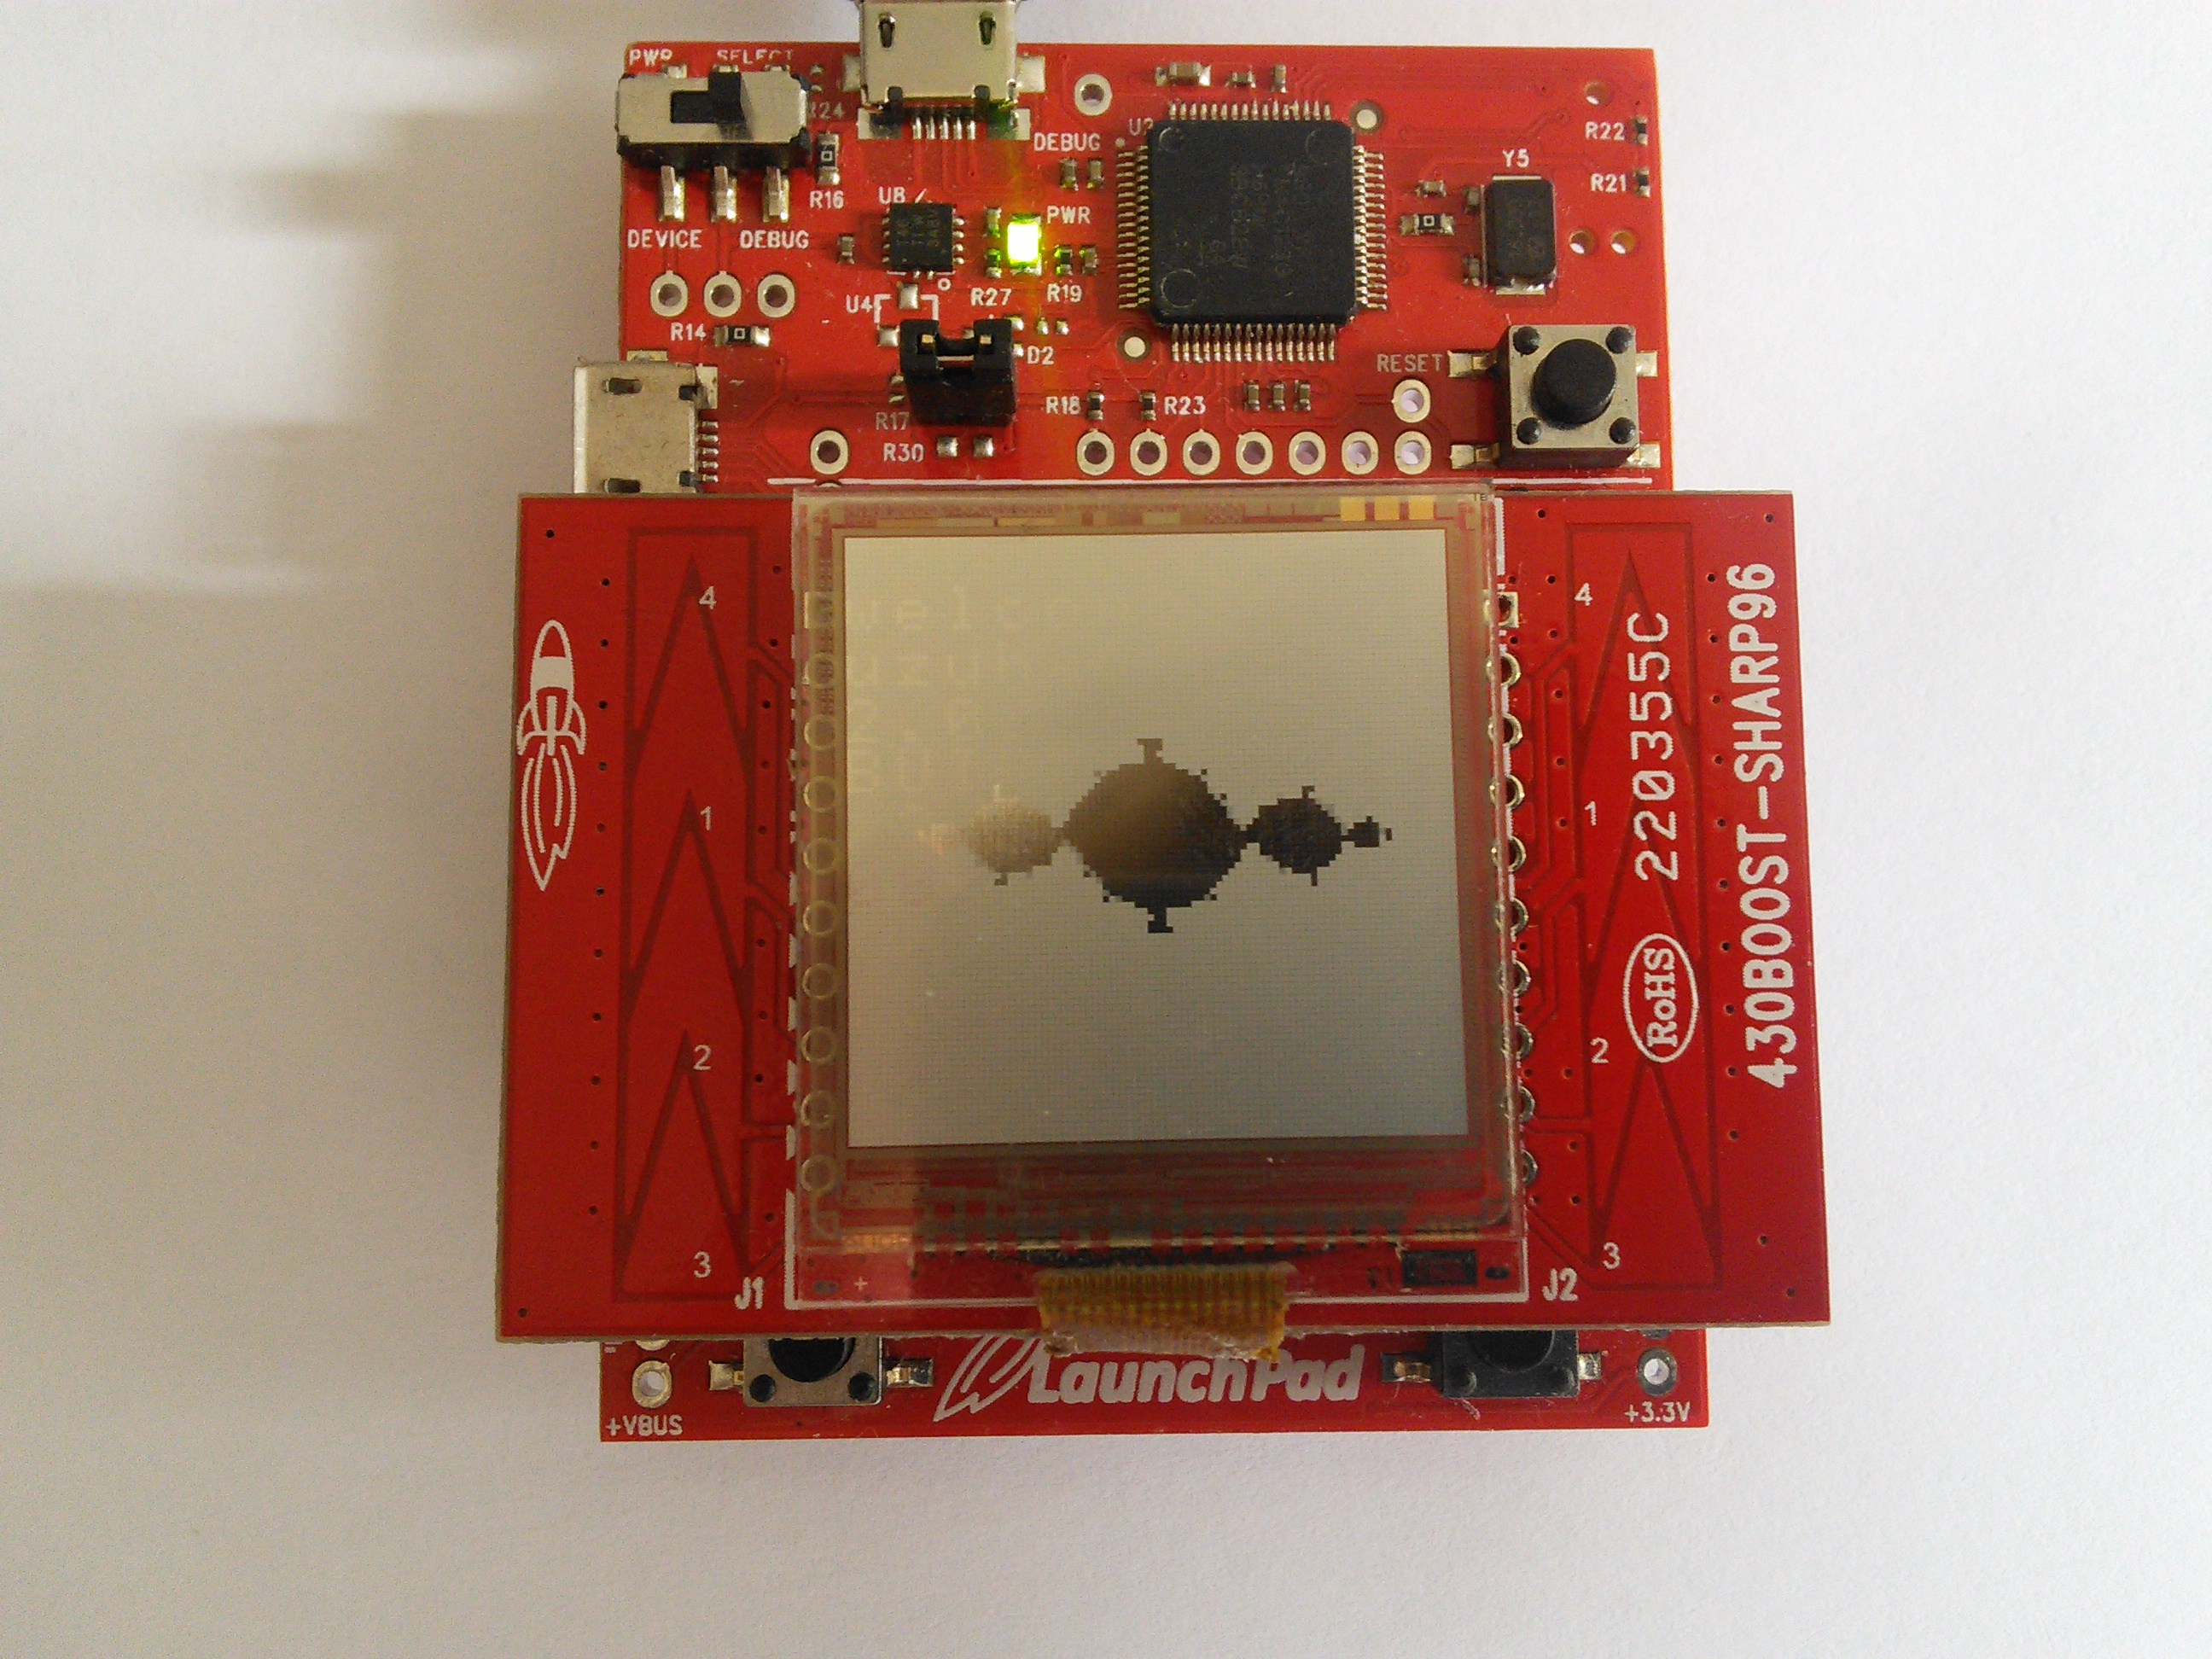
\includegraphics[width=3.0in]{testing_board_01.jpg}
\caption{TI TivaC launchpad testing board}
\label{fig_ti_launchpad}
\end{figure}

In following text, we briefly describe OS structure, and in more details priority scheduling algorithm, copared with common round robin.

\subsection{Booting process}

After microcontroller reset, HAL layer is initialized first. Especially clock confiration, gpio initialization, uart timers and adc setup.
All parts are initialized only if they are linked with. In other case, initialization of missing part is skipped.
Absolute minimum for OS running is main clock initizalization. For common problems uart and timers are necessary.\\
Next are operating system libraries initialized such stdio, software timers, messages subsystem and mutexes.

After this, kernel is initialized and user main thread is started.

\subsection{User application and libraries}

Users main loop is running in these section. Main function is called $void\ main\_thread()$. This main thread can create another threads, by calling $create\_thread$ function. Following code show how another thread can be created. When $void\ main\_thread()$ is runnig, user can inizialize it's own libraries, usually sensors, displays or communication module. Boot up and four running threads screenshot is on figure \ref{fig_os_terminal}

\noindent\begin{minipage}{.45\textwidth}
\lstset{language=C++}    
\begin{lstlisting}[frame=single, caption = thread creating]
thread_stack_t thread_01_stack
[THREAD_STACK_SIZE];

void thread_01()
{
}

void main_thread()
{
 create_thread(	thread_01, 
		thread_01_stack, 
		sizeof(thread_01_stack), 
		PRIORITY_MAX);
 while (1)
 {
 }
}
\end{lstlisting}
\end{minipage}\hfill


\begin{figure}[!t]
\centering
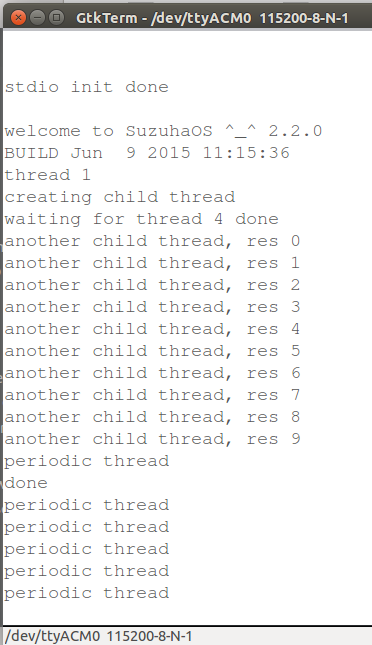
\includegraphics[width=3.0in]{threads.png}
\caption{OS terminal screenshot}
\label{fig_os_terminal}
\end{figure}

\section{Scheduling algorithm}

Main part of OS is microkernel core. Implemented is preemptive multitasking with two options : round robin scheduling, or time decrease
priority scheduler. To compare different scheduler algorithms (especially real time processing) we need first define error function. Consider threads set as
\begin{align}
\label{thread}
t_i \in T(p, k, s, d, c)
\end{align}

where
$p$ is thread priority (lower number higher priority),
$k$ is thread priority counter current value,
$s$ is thread state (running, waiting, created),
$d$ is thread deadline time (set by user, usualy in ms),
$c$ is thread running code (represented as turing machine).

Let us define thread execution time fuction as $g(t_i)$. And error function as 

\begin{align}
e = \sum_{i=1}^{Tc} |d_i - g(t_i)|
\end{align}

Where $Tc$ is threads count. This function represents error between required death time and meassured thread running time.
Using priorities we can define error as

\begin{align}
e = \sum_{i=1}^{Tc} |d_i - g(t_i)|\frac{1}{p_i}
\end{align}

Where lower $p_i$ means higher priority.

Consider than faster execution of thread isn't issue -> cpu will remaining time waiting (executing other threads or sleeping). We can write this as

\begin{align}
	 e_i &=				
	  \begin{cases}			
	   d_i - g(t_i) & if\ d_i < g(t_i) \\
	   0       & else
	  \end{cases}
\end{align}

\begin{align}
\label{error_eq}
e = \sum_{i=1}^{Tc} |e(t_i)|\frac{1}{p_i}
\end{align}

Threads with higher priority (less $p_i$) will have bigger influence on total error. To implement priorities, we define following structure for each thread.
\noindent\begin{minipage}{.45\textwidth}
\lstset{language=C++}    
\begin{lstlisting}[frame=single, caption = thread structure]
struct sThread
{
  u16 cnt, icnt;
  u32 flag; 
  u32 *sp;
};
\end{lstlisting}
\end{minipage}\hfill

Where
$cnt$ and $icnt$ are counters used for priority scheduling. Coresponding with $p$ and $k$ respectively in \ref{thread}.
When thread is created $p$ and $k$ are to $priority$ value and will remain constant (variability during execution is also posible, but not tested yet).
After each systick timer interrupt is decremented each nonzero $k$. Thread with less $k$ is choosen for next execution and it's $k$ is load back to $p$ value.
Realization in C code is presented on following code listings.

\noindent\begin{minipage}{.45\textwidth}
\lstset{language=C++}    
\begin{lstlisting}[frame=single, caption = priority scheduler]
u32 i, min_i = 0;

/*find thread with minimum cnt*/
for (i = 0; i < THREADS_MAX_COUNT; i++) 
{
 if (__thread__[i].cnt < 
     __thread__[min_i].cnt) 
   min_i=i;

/*decrement counters*/
if (__thread__[i].cnt != 0)
 __thread__[i].cnt--;
}

__thread__[min_i].cnt = 
	__thread__[min_i].icnt;
__current_thread__ = min_i;
\end{lstlisting}
\end{minipage}\hfill

For full function, there are implemented other, common functions. For thread creating, waiting or set into waiting state.

\noindent\begin{minipage}{.45\textwidth}
\lstset{language=C++}    
\begin{lstlisting}[frame=single, caption = kernel functions]

void sched_off();
void sched_on();


void yield();

u32 get_thread_id();

void kernel_init();
void kernel_start();

u32 create_thread(
	void (*thread_ptr)(), 
	thread_stack_t *s_ptr, 
	u32 stack_size, 
	u16 priority);	

void kernel_panic();

void set_wait_state();
void wake_up_threads();
void wake_up_threads_int();

void join(u32 thread_id);

\end{lstlisting}
\end{minipage}\hfill



\section{Experimental results}

For testing OS few experiments were done. First is comparsion of perfomance using hardware or software emulated float perfomance.
There were 4 running threads. One thread was caculating julia set fractal, displaying on lcd. Total calculating points was set to 96x96.
Algorithm interations was changing from interval $\langle 4, 40 \rangle$. Perfomance result is on figure \ref{fig_fpu_cpu}. In this test, basic functionalty has been tested, especially preemtive multitasking, timers and terminal interface. \\
\\
Next testing was focused on real time processing ability. There were 2 main and 6 child threads (on pictures only first 3 are shown). Each thread was waiting specified time (required waiting time) and this time was meassured. Difference, between required and meassured time is used to compare scheduling algorithms : round robin and priority scheduler. On figure \ref{fig_round_robin_scheduler_perfomance} we can see round robin result (all threads have same result). Required value is bellow measured lines, time difference was around 1ms.
On figure \label{fig_priority_scheduler_perfomance} we can see situation with priority scheduler. 

\begin{figure}[]
\centering
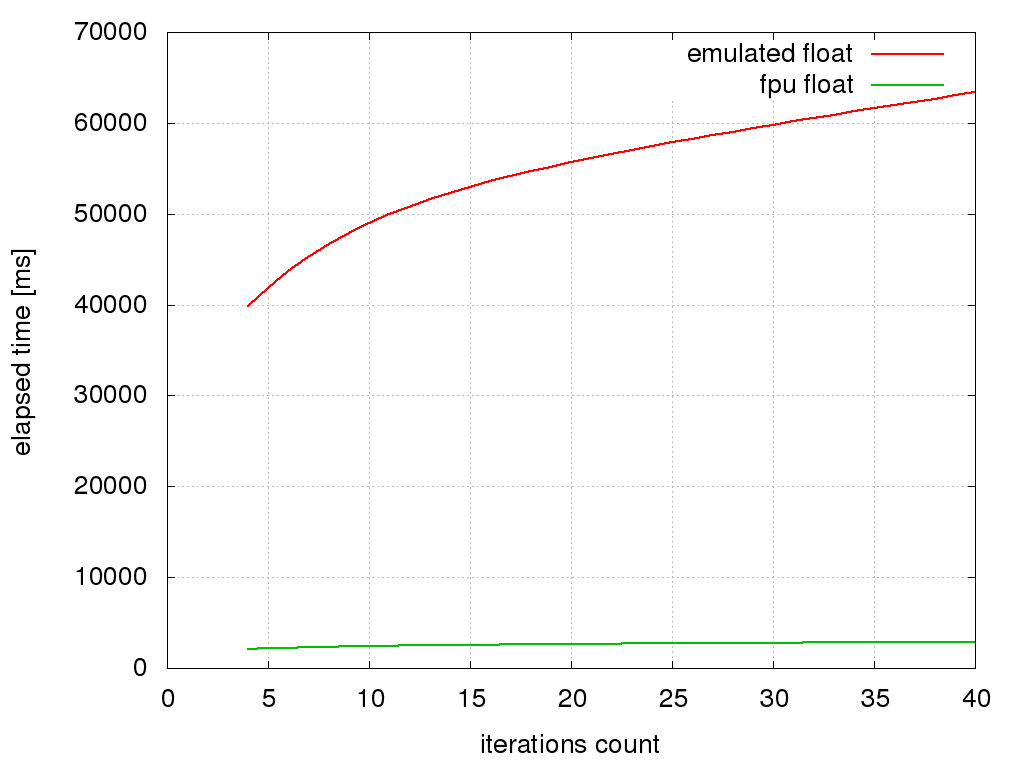
\includegraphics[width=3.0in]{fpu_cpu_performance.png}
\caption{FPU and CPU calculating times}
\label{fig_fpu_cpu}
\end{figure}


\begin{figure}[]
\centering
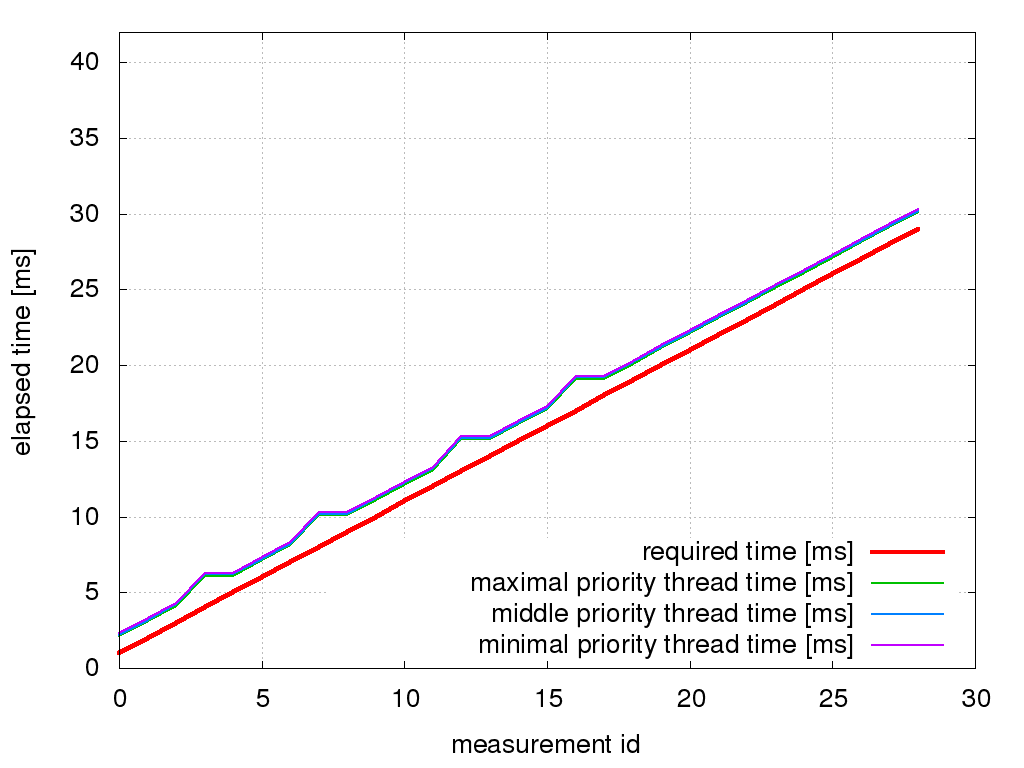
\includegraphics[width=3.0in]{round_robin_scheduler_perfomance.png}
\caption{Round robin real time test}
\label{fig_round_robin_scheduler_perfomance}
\end{figure}

\begin{figure}[]
\centering
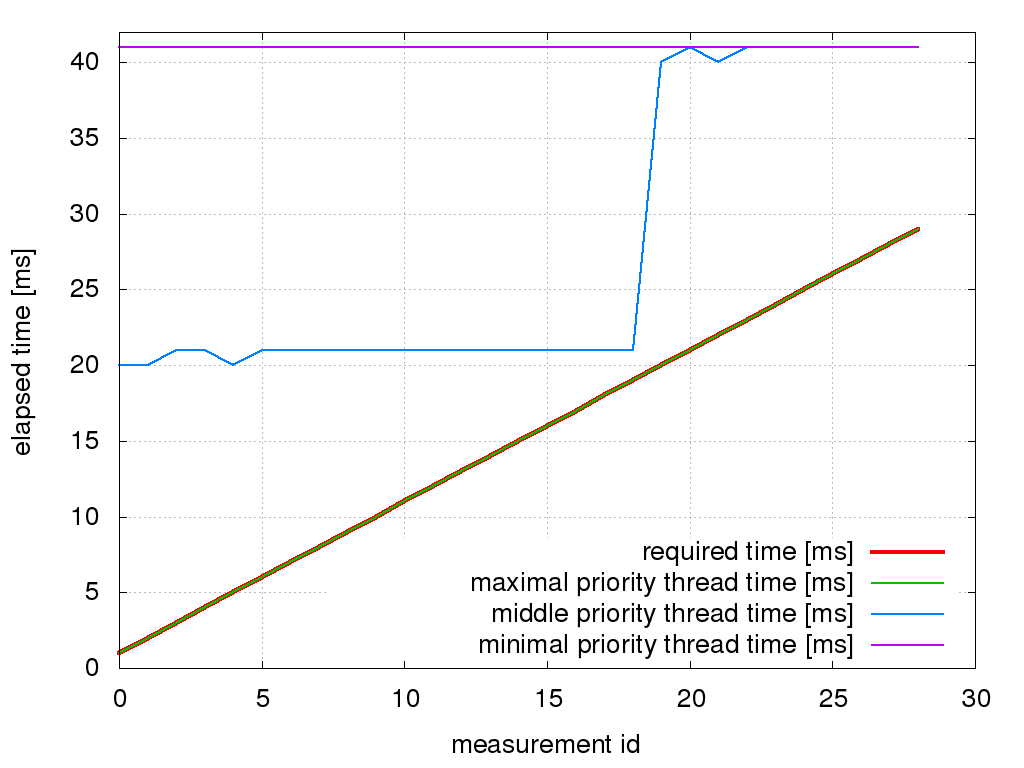
\includegraphics[width=3.0in]{priority_scheduler_perfomance.png}
\caption{Priority scheduler real time test}
\label{fig_priority_scheduler_perfomance}
\end{figure}

Threads with maximal priority perfectly meet the conditions. Threads execution time with lower priorities was executing much longer. Following priorities $p_i$ values has been used

\begin{itemize}
	\item PRIORITY\_MAX = 8		
	\item PRIORITY\_MID = 128
	\item PRIORITY\_MIN = 255
\end{itemize}

From meassured times we can using \ref{error_eq} to compute total error. Result is on figure \ref{fig_error}. From priority scheduling algorithm we can see it converges into round robin when priorities are equal, this experiment was done and results are on figure \ref{fig_priority_scheduler_similar_priority}


\begin{figure}[]
\centering
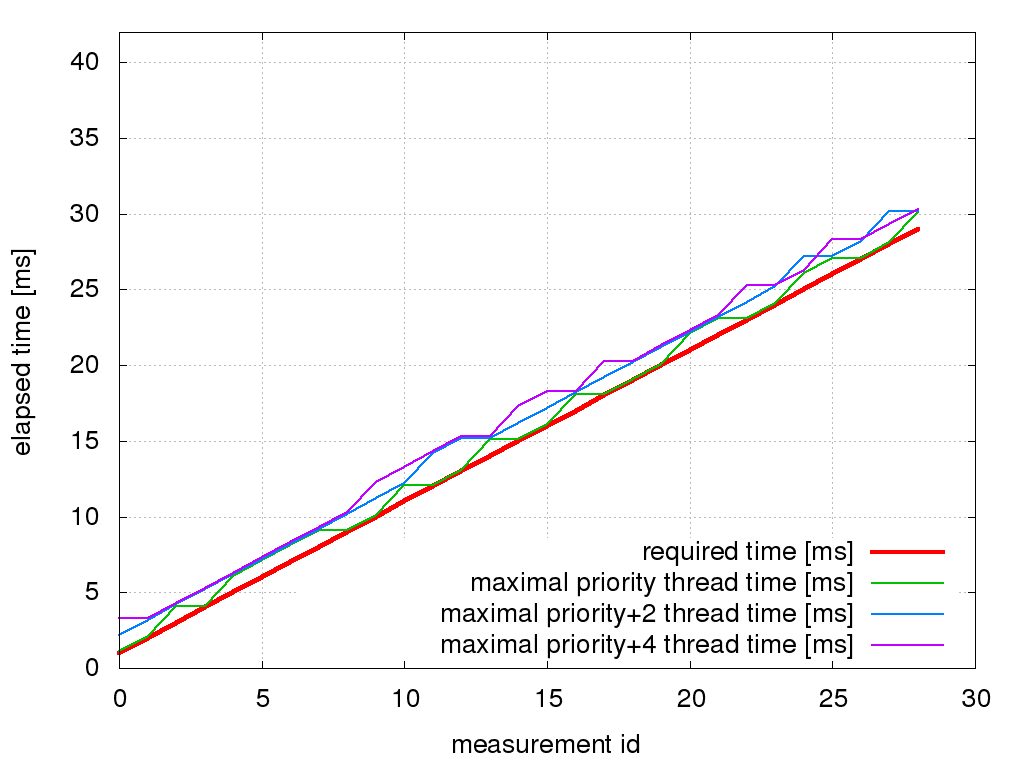
\includegraphics[width=3.0in]{priority_scheduler_similar_priority.png}
\caption{Priority scheduler real time test with similar priorities}
\label{fig_priority_scheduler_similar_priority}
\end{figure}


\begin{figure}[!b]
\centering
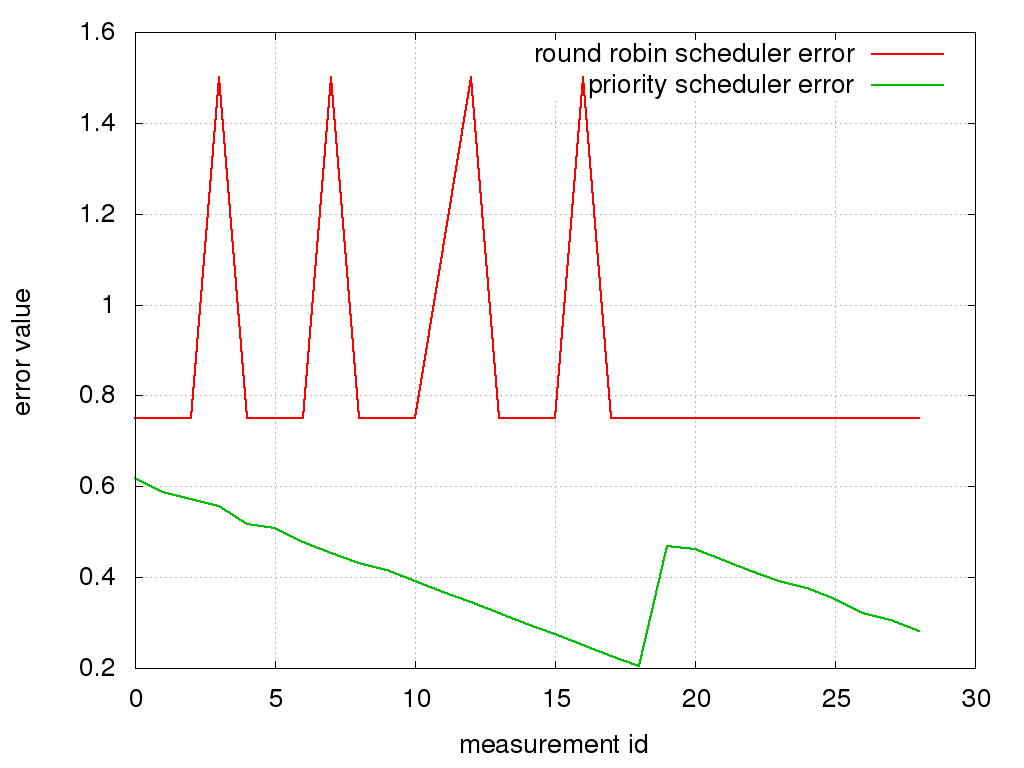
\includegraphics[width=3.0in]{scheduler_error.png}
\caption{Schedulers errors comparsion}
\label{fig_error}
\end{figure}


\section{Conclusion}
In this paper has been explaned priority scheduler and briefly introduced OS. From experimental results, we can see considering error function definition \ref{error_eq} that priority scheduler have better results. Of course, if we consider maximal deathline time without looking for priorities, better results have round robin. For applicaitons, where is necessary same priority, is round robin better solution (or priority scheduler with same priorities, figure \ref{fig_priority_scheduler_similar_priority}). For applications where is need of prioritizing some processes is of course better choice priority scheduler.



% serves to balance the column lengths on the last page of the document
% should be inserted the left column of the last page
\balance

 \bibliographystyle{plain}
\begin{thebibliography}{99}

\bibitem{Astrom:adaptive_controll}
Karl J. Astr{\"{o}}m, Dr. Bj{\"{o}}rn Wittenmark, Adaptive Control: Second Edition, ISBN10 100486462781

\bibitem{Colorado:closed_loop}
MAE171B DIGITAL CONTROL OF PHYSICAL SYSTEMS, H. Peng and George T.-C Chiu, T-C. Tsao ©1994- 2008, http://ecee.colorado.edu/shalom/Emulations.pdf

\bibitem{VogelEdgar:controller}
Vogel, E.F, and T.F. Edgar, A New Dead Time Compensator for Digital Control, lSA/80 Proc., Houston, TX, Oct. 1980.

\bibitem{LMS:normalised}
Normalised LMS, Note by Y. Hua , http://www.ee.ucr.edu/~yhua/ee211/Note\_3.pdf

\bibitem{Springer:adaptive_filtering}
Apolinario jr, Jose Antonio (Ed.),  QRD-RLS Adaptive Filtering, ISBN 978-0-387-09734-3, 2009, chap 2

\bibitem{TI:msp430}
Texas Instruments, Launchpad http://www.ti.com/tool/msp-exp430g2
\end{thebibliography}




\end{document}
